\documentclass[12pt]{article}
\usepackage{amsmath,amsthm,amssymb,amsfonts,setspace}
\usepackage{pgf-umlcd}
\usepackage{tikz}
\usetikzlibrary{arrows.meta, shapes.multipart, positioning}
\textwidth 7.0 truein
\oddsidemargin -0.25in   %left-hand edge
\evensidemargin -0.5 truein  %right-hand edge
\topmargin -0.85in      %top of paper to top of head, pulls whole unit
\textheight 9.5in
\usepackage[margin=1in]{geometry}
\usepackage{fancyvrb}
\usepackage[T1]{fontenc}
%%%% In most cases you won't need to edit anything above this line %%%%

\begin{document}
{\raggedleft{} 523c0012 - Huynh Nhat Huy \\   Data Structures And Algorithms 2025 - 2026  \\  LAB 5: Review \\ Homework Assignment \\}
\vspace{20pt}
\textbf{1. INTRODUCTION}\\\\
The objective of this lab is to comprehensively review core data structures and algorithms, including Linked Lists, Stacks, Queues, Recursion, and Sorting, in preparation for the midterm examination. The first exercise requires implementing an integer-based Linked List following the provided UML model:
\\
\begin{center}
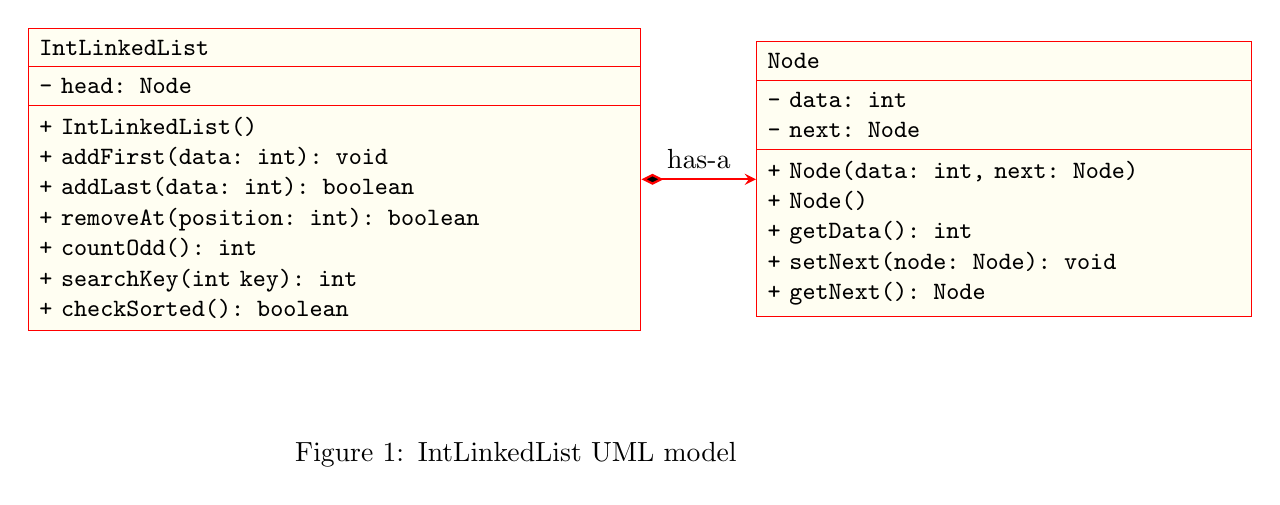
\begin{tikzpicture}[    % define 'Method' here
    umlbox/.style={
        draw=red, 
        fill=yellow!5, 
        rectangle split, 
        rectangle split parts=3, 
        inner sep=4pt, 
        text width=6.5cm,
        font=\small\ttfamily
    }
]   

    % 1. The LinkedList
    \node [umlbox, text width=7.5cm] (IntList) at (0,7) {
        \centering \textbf{IntLinkedList}
        \nodepart{second}
        - head: Node
        \nodepart{third}
        + IntLinkedList() \\
        + addFirst(data: int): void \\
        + addLast(data: int): boolean \\
        + removeAt(position: int): boolean \\
        + countOdd(): int \\
        + searchKey(int key): int \\
        + checkSorted(): boolean
    };

    % 2. The Node
    \node [umlbox, text width=6cm] (Node) at (8.5,7) {
        \centering \textbf{Node}
        \nodepart{second}
        - data: int \\
        - next: Node
        \nodepart{third}
        + Node(data: int, next: Node) \\
        + Node() \\
        + getData(): int \\
        + setNext(node: Node): void \\
        + getNext(): Node
    };

    % The Connections
    % The 'Has-a' Composition Arrow
    \draw [red, {Diamond[fill=black]}-stealth, thick] (IntList.east) -- (Node.west) 
        node[midway, sloped, above, black] {has-a};

    % 3. The "Manual" Caption 
    \node [text width=10cm] at (4.5, 3.5) {Figure 1: IntLinkedList UML model};

\end{tikzpicture}
\end{center}

\begin{description}
    \item[Node:] Represents a single item in the list, containing integer data and a reference to the next node.
    \item[IntLinkedList:] The core class that manages the sequence of Nodes and handles insertion, deletion, and searching.
\end{description}

%------------------------------------------------------------------------------------------------------%

\textbf{2. EXERCISES}
\begin{itemize}

\item[\textbf{Exercise 1. }] \textbf{Linked List Implementation} \\
The foundational `Node` and `IntLinkedList` classes were implemented from scratch. Below is the implementation for the initialization, adding to the front of the list, and appending to the end while checking for duplicate values:
\begin{verbatim}
    // IntLinkedList.java
    public class IntLinkedList {
        private Node head;

        public IntLinkedList() {
            this.head = null;
        }

        public void addFirst(int data) {
            Node newNode = new Node(data, this.head); 
            this.head = newNode;
        }
        
        public boolean addLast(int data) {
            if (head == null) {
                addFirst(data);
                return true;
            }
            Node current = head;
            while (current.getNext() != null) {
                if (current.getData() == data) return false; // Duplicate check
                current = current.getNext();
            }
            if (current.getData() == data) return false; // Check last node
            
            current.setNext(new Node(data, null));
            return true;
        }
    }
\end{verbatim}

\item[\textbf{Exercise 2. }] \textbf{Stack and Queue Operations} \\
Custom `MyStack` and `MyQueue` structures were utilized to solve practical evaluation problems. 

First, a Stack was used to evaluate postfix mathematical expressions:
\begin{verbatim}
    // PostfixCalculator.java
    public static int calculatePostfix(String s) {
        MyStack<String> stack = new MyStack<>();
        String[] split_ch = s.split(" "); 
        
        for (String ch : split_ch) {
            if (ch.equals("+") || ch.equals("-") || ch.equals("*") || ch.equals("/")) {
                int a = Integer.parseInt(stack.pop());
                int b = Integer.parseInt(stack.pop());
                int res = 0;
                switch (ch) {
                    case "+": res = b + a; break;
                    case "-": res = b - a; break;
                    case "*": res = b * a; break;
                    case "/": res = b / a; break;
                }
                stack.push(String.valueOf(res)); 
            } else {
                stack.push(ch);
            }
        }
        return Integer.parseInt(stack.pop());
    }
\end{verbatim}

Second, both data structures were combined to verify if a positive integer is a palindrome by comparing LIFO and FIFO extractions:
\begin{verbatim}
    // PalindromeChecker.java
    public static boolean isPalindrome(int n) {
        String strN = String.valueOf(n);
        MyStack<Character> stack = new MyStack<>();
        MyQueue<Character> queue = new MyQueue<>();
        
        for (char c : strN.toCharArray()) {
            stack.push(c);
            queue.enQueue(c);
        }
        
        while (!stack.isEmpty() && !queue.isEmpty()) {
            if (stack.pop() != queue.deQueue()) {
                return false; 
            }
        }
        return true; 
    }
\end{verbatim}

\item[\textbf{Exercise 3. }] \textbf{Recursion} \\
Various mathematical and structural problems were solved using both recursive and iterative approaches. For example, computing mathematical summations requires distinct logic depending on the approach:
\begin{verbatim}
    // Recursive Summation: sum((x+1)/2) from x=0 to n
    public static double sumA_recur(int n) {
        if (n == 0) return 1.0 / 2.0; 
        return (n + 1) / 2.0 + sumA_recur(n - 1);
    }

    // Iterative Summation equivalent
    public static double sumA_iter(int n) {
        double sum = 0;
        for (int x = 0; x <= n; x++) {
            sum += (x + 1) / 2.0;
        }
        return sum;
    }
\end{verbatim}
Additionally, piecewise functions such as the Fibonacci sequence were implemented recursively:
\begin{verbatim}
    // Recursion: Fibonacci piecewise function
    public static int funcD_recur(int n) {
        if (n == 0) return 0;
        if (n == 1) return 1;
        return funcD_recur(n - 1) + funcD_recur(n - 2);
    }
\end{verbatim}

\item[\textbf{Exercise 4. }] \textbf{Sorting Algorithms} \\
Selection Sort, Bubble Sort, and Insertion Sort were implemented. A print function was added to the outer loop of each algorithm to display the array's state step-by-step as required by the assignment constraints.
\begin{verbatim}
    // Selection Sort Implementation
    public static void selectionSort(int[] a) {
        int n = a.length;
        for (int i = 0; i < n - 1; i++) {
            int minIndex = i;
            for (int j = i + 1; j < n; j++) {
                if (a[j] < a[minIndex]) {
                    minIndex = j;
                }
            }
            int temp = a[minIndex];
            a[minIndex] = a[i];
            a[i] = temp;
            
            printArray(a); // Output state per requirement
        }
    }

    // Bubble Sort Implementation
    public static void bubbleSort(int[] a) {
        int n = a.length;
        for (int i = 0; i < n - 1; i++) {
            for (int j = 0; j < n - i - 1; j++) {
                if (a[j] > a[j + 1]) {
                    int temp = a[j];
                    a[j] = a[j + 1];
                    a[j + 1] = temp;
                }
            }
            printArray(a); // Output state per requirement
        }
    }
\end{verbatim}

\end{itemize}

That's the end of my report, thank you for reading. \\\\
\textbf{3. AFTERWORDS}\\\\

\centering
\vspace{20pt}

GitHub repository link containing all of my DSA lab files, including source codes, \\ and reports in .PDF and .TEX:\\ https://github.com/Thundercok/dump/tree/main/DSA
\end{document}